\documentclass[tikz,border=4pt]{standalone}
\usepackage{amsmath}
\usepackage{xcolor}
\usetikzlibrary{arrows.meta,positioning}

\begin{document}
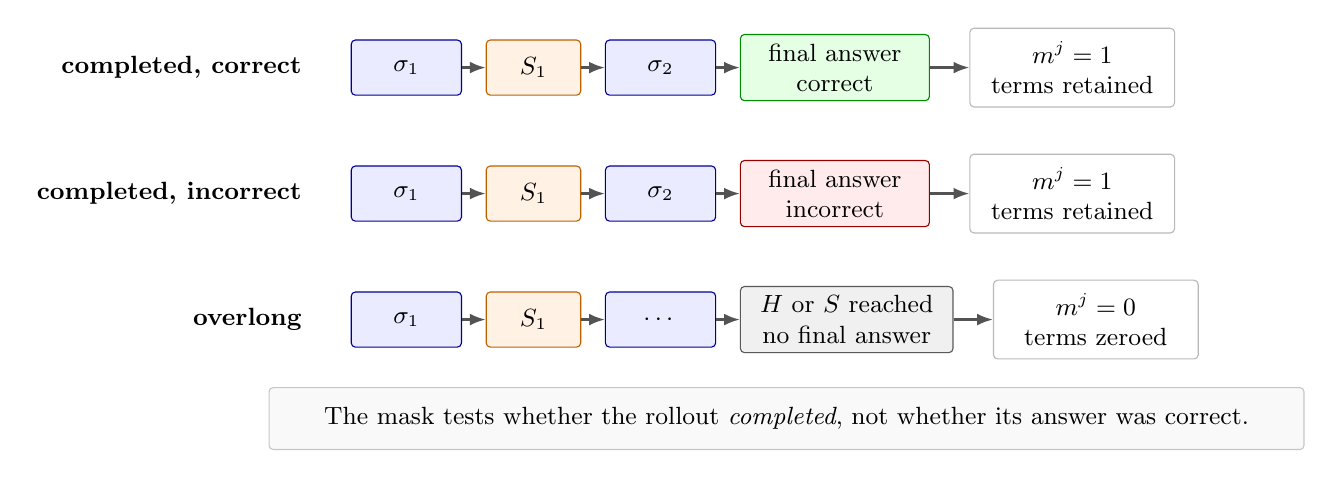
\begin{tikzpicture}[
  font=\small,
  flow/.style={-{Latex[length=2mm]}, thick, draw=gray!65!black},
  segment/.style={
    draw=blue!60!black,
    fill=blue!8,
    rounded corners=1.5pt,
    minimum width=14mm,
    minimum height=7mm,
    align=center
  },
  summary/.style={
    draw=orange!75!black,
    fill=orange!10,
    rounded corners=1.5pt,
    minimum width=12mm,
    minimum height=7mm,
    align=center
  },
  finalgood/.style={
    draw=green!55!black,
    fill=green!10,
    rounded corners=1.5pt,
    minimum width=24mm,
    minimum height=7mm,
    align=center
  },
  finalbad/.style={
    draw=red!60!black,
    fill=red!8,
    rounded corners=1.5pt,
    minimum width=24mm,
    minimum height=7mm,
    align=center
  },
  limit/.style={
    draw=gray!70!black,
    fill=gray!12,
    rounded corners=1.5pt,
    minimum width=27mm,
    minimum height=7mm,
    align=center
  },
  result/.style={
    draw=gray!55,
    fill=white,
    rounded corners=1.5pt,
    minimum width=26mm,
    minimum height=10mm,
    align=center
  },
  rowlabel/.style={anchor=east, align=right, font=\small\bfseries}
]

\node[rowlabel] (label1) at (0,1.6) {completed, correct};
\node[segment, right=5mm of label1] (a1) {$\sigma_1$};
\node[summary, right=3mm of a1] (s1) {$S_1$};
\node[segment, right=3mm of s1] (a2) {$\sigma_2$};
\node[finalgood, right=3mm of a2] (f1) {final answer\\correct};
\node[result, right=5mm of f1] (r1) {$m^j=1$\\terms retained};
\draw[flow] (a1) -- (s1);
\draw[flow] (s1) -- (a2);
\draw[flow] (a2) -- (f1);
\draw[flow] (f1) -- (r1);

\node[rowlabel] (label2) at (0,0) {completed, incorrect};
\node[segment, right=5mm of label2] (b1) {$\sigma_1$};
\node[summary, right=3mm of b1] (s2) {$S_1$};
\node[segment, right=3mm of s2] (b2) {$\sigma_2$};
\node[finalbad, right=3mm of b2] (f2) {final answer\\incorrect};
\node[result, right=5mm of f2] (r2) {$m^j=1$\\terms retained};
\draw[flow] (b1) -- (s2);
\draw[flow] (s2) -- (b2);
\draw[flow] (b2) -- (f2);
\draw[flow] (f2) -- (r2);

\node[rowlabel] (label3) at (0,-1.6) {overlong};
\node[segment, right=5mm of label3] (c1) {$\sigma_1$};
\node[summary, right=3mm of c1] (s3) {$S_1$};
\node[segment, right=3mm of s3] (c2) {$\cdots$};
\node[limit, right=3mm of c2] (f3) {$H$ or $S$ reached\\no final answer};
\node[result, right=5mm of f3] (r3) {$m^j=0$\\terms zeroed};
\draw[flow] (c1) -- (s3);
\draw[flow] (s3) -- (c2);
\draw[flow] (c2) -- (f3);
\draw[flow] (f3) -- (r3);

\node[
  draw=gray!45,
  fill=gray!5,
  rounded corners=1.5pt,
  inner xsep=7mm,
  inner ysep=2mm,
  below=5mm of c2,
  xshift=16mm
] {\strut The mask tests whether the rollout \emph{completed}, not whether its answer was correct.};

\end{tikzpicture}
\end{document}
